\documentclass{article}

\usepackage[utf8]{inputenc}
\usepackage[spanish]{babel}
\usepackage{geometry}
\usepackage{graphicx}
\usepackage{titlesec}
\usepackage{lipsum}
\usepackage[dvipsnames]{xcolor}
\usepackage[fleqn]{mathtools}
\usepackage{booktabs}
\usepackage{amsmath}
\usepackage{latexsym}
\usepackage{nccmath}
\usepackage{multicol}
\usepackage{listings}
\usepackage{tasks}
\usepackage{color}
\usepackage{float}
\usepackage{enumitem}
\usepackage{longtable}
\usepackage{makecell}
\usepackage{caption}
\usepackage[parfill]{parskip}
\usepackage{lipsum}
\usepackage{enumitem}
\usepackage{hyperref}% Para manejar enlaces
\usepackage{fancyhdr}
\usepackage{adjustbox}
\usepackage{amsmath}
\usepackage{tocloft}
\usepackage{soul}

%Definicion de colores
\definecolor{colorIPN}{rgb}{0.5, 0.0,0.13}
\definecolor{colorESCOM}{rgb}{0.0, 0.5,1.0}
\definecolor{myorange}{RGB}{255, 204, 153}
\graphicspath{ {imagenes/} }
%Configuraciones extras de colores
\definecolor{codegreen}{rgb}{0,0.6,0}
\definecolor{codered}{rgb}{0.6,0,0}
\definecolor{codegray}{rgb}{0.5,0.5,0.5}
\definecolor{codepurple}{rgb}{0.58,0,0.82}
\definecolor{backcolour}{rgb}{0.95,0.95,0.92}

% Configuración de la portada
\titleformat{\section}[block]{\normalfont\huge\bfseries}{\thesection}{1em}{}
\geometry{a4paper, margin=1in}

% Definir comandos para información repetitiva
\newcommand{\logoInstitucion}{logotipo_ipn.png} % Reemplaza con el nombre del archivo de tu logo
\newcommand{\logoUniversidad}{EscudoESCOM.png} % Reemplaza con el nombre del archivo de tu logo
\newcommand{\nombreInstituto}{Instituto Politecnico Nacional}
\newcommand{\facultad}{Escuela Superior de Computo}
\newcommand{\materia}{Teoría de la Computación}
\newcommand{\grupo}{5BM1}
\newcommand{\profesora}{Genaro Juarez Martínez}
\newcommand{\periodo}{2024/02}
\newcommand{\alumno}{Carrillo Barreiro José Emiliano}

% Definir nuevas listas para información repetitiva
\newlist{bracketed}{enumerate}{1}
\setlist[bracketed,1]{label={[{\arabic*}]},left=0pt}

% Configuración del encabezado y pie de página
\pagestyle{fancy}
\fancyhf{} % Limpia todos los campos

% Encabezado
\fancyhead[C]{\textbf{\nombreInstituto\\ \facultad}}
\fancyhead[L]{
\includegraphics[width=1cm]{logotipo_ipn.png}}
\fancyhead[R]{
\includegraphics[width=1.5cm]{EscudoESCOM.png}}

% Pie de página
\fancyfoot[C]{\materia||\grupo\\ \alumno\\ \thepage}

% Configuración del grosor de la línea en el encabezado y pie de página
\renewcommand{\headrulewidth}{0.4pt}
\renewcommand{\footrulewidth}{0.4pt}

% Ajuste del tamaño del encabezado
\setlength{\headheight}{34.0845pt}
\addtolength{\topmargin}{-22.0845pt}

% Configuración de lstlisting para Python
\lstdefinestyle{mystyle}{
    backgroundcolor=\color{backcolour},
    commentstyle=\color{codegreen},
    keywordstyle=\color{codepurple},
    numberstyle=\tiny\color{codegray},
    stringstyle=\color{codered},
    basicstyle=\ttfamily\small,
    breakatwhitespace=false,
    breaklines=true,
    captionpos=b,
    keepspaces=true,
    numbers=left,
    numbersep=5pt,
    showspaces=false,
    showstringspaces=false,
    showtabs=false,
    tabsize=2
}

\lstdefinestyle{custompython}{
    language=Python,
    basicstyle=\small\ttfamily,
    keywordstyle=\color{blue},
    stringstyle=\color{green},
    commentstyle=\color{red},
    numbers=left,
    numberstyle=\tiny\color{gray},
    stepnumber=1,
    numbersep=5pt,
    backgroundcolor=\color{white},
    frame=single,
    captionpos=b,
    breaklines=true,
    breakatwhitespace=false,
    showstringspaces=false,
    morekeywords={import,plt,np,ws,y,gradient}
}

\lstdefinestyle{cppstyle}{
    language=C++,
    basicstyle=\small\ttfamily,
    keywordstyle=\color{blue},
    commentstyle=\color{green!40!black},
    stringstyle=\color{orange},
    showstringspaces=false,
    breaklines=true,
    breakatwhitespace=true,
    numbers=left,
    numberstyle=\tiny,
    stepnumber=1,
    numbersep=5pt,
    frame=single,
    captionpos=b,
    backgroundcolor=\color{gray!5},
    xleftmargin=0.5cm,
    xrightmargin=0.5cm
}

% Definición de estilo para MATLAB
\lstdefinestyle{matlabstyle}{
    language=Matlab,
    basicstyle=\small\ttfamily,
    keywordstyle=\color{blue},
    commentstyle=\color{green!40!black},
    stringstyle=\color{purple!50!blue!50!white},
    showstringspaces=false,
    breaklines=true,
    breakatwhitespace=true,
    numbers=left,
    numberstyle=\tiny,
    stepnumber=1,
    numbersep=5pt,
    frame=single,
    captionpos=b,
    backgroundcolor=\color{gray!5},
    xleftmargin=0.5cm,
    xrightmargin=0.5cm
}

% Personalización del índice de listados
\newcommand{\listcppname}{Índice de Listados de C++}
\newcommand{\listmatlabname}{Índice de Listados de MATLAB}
\newlistof{cpplistings}{lolcpp}{\listcppname}
\newlistof{matlablistings}{lolmatlab}{\listmatlabname}

% Configuración para los listados de C++
\lstset{style=cppstyle}
\newcommand{\cpplisting}[1]{%
    \refstepcounter{cpplistings}%
    \addcontentsline{lolcpp}{cpplistings}{\protect\numberline{\thecpplistings}#1}\par}

% Configuración para los listados de MATLAB
\lstset{style=matlabstyle}
\newcommand{\matlablisting}[1]{%
    \refstepcounter{matlablistings}%
    \addcontentsline{lolmatlab}{matlablistings}{\protect\numberline{\thematlablistings}#1}\par}

\begin{document}

% Portada
\begin{titlepage}
    \begin{center}
        \vspace*{1cm}

        \includegraphics[width=0.25\textwidth]{\logoInstitucion}

        \vspace{1cm}

        \textbf{\LARGE \nombreInstituto} \\
        \textbf{\Large \facultad} \\
        \vspace{0.5cm}
        \textbf{\large Materia: \materia} \\
        \textbf{\large Grupo: \grupo} \\
        \vspace{0.5cm}
        \textbf{\large Profesor: \profesora} \\
        \textbf{\large Periodo: \periodo} \\

        \vspace{1cm}

        \textbf{\LARGE Practica 02:} \\
        \vspace{0.5cm}
        \textbf{\Large Automáta finito no determinista (AFN) detector de cadenas binarias con terminacion <<01>>} \\

        \vfill

        \textbf{\large Realizado por:} \\
        \textbf{\large \alumno}

        \vspace{1cm}

        \includegraphics[width=0.4\textwidth]{\logoUniversidad}

        \vspace{1cm}

        \textbf{\large \facultad} \\
        \textbf{\large Fecha: \today}

    \end{center}
\end{titlepage}

% Índice
\tableofcontents
\newpage
\listofcpplistings%Crea indice de codigos en C++
\listofmatlablistings%Crea indice de codigos en MATLAB
%\listoftables
\listoffigures
\newpage

\section{Resumen.}
En la Práctica 02, nos adentramos en el mundo de los autómatas no deterministas para la detección de cadenas binarias con terminación
\textit{01}. Comenzamos implementando un autómata no determinista en un lenguaje de programación C++, para posteriormente hacer la
animacion en Matlab. Este autómata se diseña para reconocer cadenas binarias que finalizan con \textit{01}. El programa solicita al
usuario que ingrese una cadena binaria y luego evalúa si cumple con la condición especificada por el autómata.

El proceso implica la definición de los estados del autómata, las transiciones entre estos estados y el manejo de la entrada del
usuario para determinar si la cadena ingresada es aceptada o rechazada por el autómata. Este enfoque permite comprender cómo funcionan
los autómatas no deterministas y cómo se pueden utilizar para resolver problemas específicos, en este caso, la detección de ciertos
patrones en cadenas binarias.

\section{Introducción.}
Este informe detalla la implementación de un autómata no determinista para la detección de cadenas binarias con terminación \textit{01},
utilizando los lenguajes de programación C++ y MATLAB.\@ Nos centraremos en los principios fundamentales de la teoría de autómatas,
explorando cómo estos conceptos se aplican en la creación de un autómata capaz de reconocer patrones específicos en cadenas binarias.

El objetivo principal es comprender cómo los autómatas no deterministas pueden ser diseñados e implementados en un entorno
computacional utilizando C++ y MATLAB.\@ Para ello, nos sumergiremos en conceptos como estados, transiciones, alfabetos y la estructura
de las cadenas binarias. Esta comprensión teórica proporcionará la base necesaria para desarrollar un autómata capaz de identificar
cadenas binarias que terminan con \textit{01}.

Al combinar la teoría de autómatas con las capacidades de programación de C++ y MATLAB, no solo buscamos crear un autómata funcional, sino también profundizar en nuestra comprensión de los principios subyacentes que gobiernan su comportamiento. Este enfoque integral nos permitirá no solo resolver problemas específicos relacionados con la detección de patrones en cadenas binarias, sino también sentar las bases para abordar problemas más complejos en el ámbito de la informática teórica.

\section{Marco Teorico.}
    \subsection{Teoría de Automátas.}
        \begin{quote}
            La teoría de autómatas es un campo fundamental en la ciencia de la computación que se ocupa del estudio de dispositivos
            abstractos de cálculo. Estos dispositivos, conocidos como \textit{máquinas}, son modelos matemáticos que nos permiten entender y
            analizar el comportamiento de sistemas computacionales. Desde sus primeros pasos en la década de 1930 con los trabajos de
            Alan Turing, la teoría de autómatas ha evolucionado y se ha ramificado en diversos aspectos que abarcan desde autómatas finitos
            simples hasta conceptos más complejos como gramáticas formales y problemas computacionales.

            El punto de partida de la teoría de autómatas se encuentra en los estudios de Turing sobre las \textit{máquinas de Turing},
            dispositivos abstractos capaces de realizar cualquier cálculo computacional. Turing propuso estas máquinas como un modelo universal
            de computación, estableciendo así los fundamentos teóricos de lo que hoy entendemos como computación. A partir de este trabajo pionero,
            otros investigadores comenzaron a explorar variantes más simples de las máquinas de Turing, dando lugar a los autómatas finitos.

            Los autómatas finitos son modelos computacionales simples que representan sistemas con un número limitado de estados y una capacidad
            limitada de procesamiento. Estos dispositivos se utilizan para modelar sistemas de control, reconocer patrones en cadenas de
            símbolos y resolver problemas de decisión. Además, los autómatas finitos están estrechamente relacionados con las gramáticas
            formales, ya que ambos se utilizan para describir y generar lenguajes formales.

            La teoría de autómatas también abarca el estudio de problemas computacionales y la clasificación de su complejidad. Investigadores
            como Stephen Cook han contribuido significativamente al campo al desarrollar técnicas para clasificar los problemas en función de
            su dificultad computacional. Esta clasificación ha llevado a la identificación de problemas que pueden resolverse eficientemente y
            problemas que son inherentemente difíciles de resolver.\cite{hopcroft2007introduccion}
        \end{quote}

    \subsection{Alfabetos.}
        \begin{quote}
            Un alfabeto, representado convencionalmente por el símbolo $\Sigma$, es un conjunto finito y no vacío de símbolos.
            Estos símbolos pueden ser números, letras, caracteres especiales, o cualquier otro tipo de elemento que se utilice para formar
            cadenas de caracteres. Algunos ejemplos comunes de alfabetos incluyen:

            \begin{enumerate}
                \item $\Sigma=\{0,1\}$: el alfabeto binario, utilizado en sistemas informáticos para representar datos de manera binaria.
                \item $\Sigma=\{a,b,\ldots,z\}$: el conjunto de todas las letras minúsculas del alfabeto latino.
                \item El conjunto de todos los caracteres ASCII o el conjunto de todos los caracteres ASCII imprimibles, utilizado en programación y comunicaciones
                para representar texto y caracteres especiales.\cite{hopcroft2007introduccion}
            \end{enumerate}
        \end{quote}
    \subsection{Cadena de caracteres.}
        \begin{quote}
            Una cadena de caracteres, también conocida como palabra en algunos contextos, es una secuencia finita de símbolos seleccionados de
            un alfabeto específico. Por ejemplo, la cadena <<01101>> es una cadena del alfabeto binario $\Sigma = \{0,1\}$, mientras que <<hola>>
            es una cadena del alfabeto de letras minúsculas del alfabeto latino. Incluso la cadena vacía, representada por $\varepsilon$, es
            una cadena que puede construirse en cualquier alfabeto.\cite{hopcroft2007introduccion}
        \end{quote}

    \subsection{Longitud de cadenas.}
        \begin{quote}
            La longitud de una cadena se refiere al número de símbolos que contiene. Por ejemplo, la cadena <<01101>> tiene una longitud
            de 5, mientras que la cadena vacía tiene una longitud de 0. La notación estándar para indicar la longitud de una cadena $w$
            es $|w|$. Por lo tanto, $|01101| = 5$ y $|\varepsilon| = 0$.\cite{hopcroft2007introduccion}
        \end{quote}

    \subsection{Autómatas Finitos No Deterministas (AFN)}

    \begin{quote}
        Los autómatas finitos no deterministas (AFN) son una clase de autómatas que poseen la capacidad de estar en varios estados
        simultáneamente. Esta característica se manifiesta en la capacidad del autómata para ``conjeturar'' sobre su entrada en ciertos
        momentos durante su procesamiento. Por ejemplo, al buscar determinadas secuencias de caracteres, como palabras clave, dentro de
        una cadena de texto extensa, el AFN puede ``conjeturar'' el inicio de una de estas cadenas y emplear una serie de estados para
        verificar la presencia de la cadena, carácter por carácter.\cite{hopcroft2007introduccion}
    \end{quote}

        \subsubsection{Aplicaciones de los AFN}

        Un ejemplo claro de la aplicación de los AFN se encuentra en la búsqueda de patrones en texto, como la búsqueda de palabras clave
        o la validación de formatos específicos. Además, los AFN se utilizan en el análisis léxico de compiladores, donde se emplean para
        reconocer tokens en un programa fuente.

\section[Desarrollo]{Desarrollo de la Practica.}
    \subsection[Especificaciones]{información del sistema.}
    La siguiente información fue extraida gracias al comando \texttt{systeminfo} en \texttt{cmd}: %tambien se puede usa dixdiag
        \begin{lstlisting}[language={},basicstyle=\ttfamily\footnotesize]
Nombre de host:                            CARBAJE
Nombre del sistema operativo:              Microsoft Windows 11 Home
Version del sistema operativo:             10.0.22631 N/D Compilacion 22631
Fabricante del sistema operativo:          Microsoft Corporation
Configuracion del sistema operativo:       Estacion de trabajo independiente
Tipo de compilacion del sistema operativo: Multiprocessor Free
Propiedad de:                              emi.cruzazul@hotmail.com
Organizacion registrada:
Fecha de instalacion original:             04/03/2024, 8:09:03
Tiempo de arranque del sistema:            12/03/2024, 9:41:56
Fabricante del sistema:                    GIGABYTE
Modelo el sistema:                         G5 KF5
Tipo de sistema:                           x64-based PC
Procesador(es):                            1 Procesadores instalados.
                                            [01]: Intel64 Family 6 Model 186 Stepping 2 GenuineIntel ~2400 Mhz
Version del BIOS:                          INSYDE Corp. FD06, 03/11/2023
Directorio de Windows:                     C:\Windows
Directorio de sistema:                     C:\Windows\system32
Dispositivo de arranque:                   \Device\HarddiskVolume1
Configuracion regional del sistema:        es;Espanol (internacional)
Idioma de entrada:                         en-us;Ingles (Estados Unidos)
Zona horaria:                              (UTC-06:00) Guadalajara, Ciudad de Mexico, Monterrey
Cantidad total de memoria fisica:          16.088 MB
Memoria fisica disponible:                 7.991 MB
Memoria virtual: tamano maximo:            65.240 MB
Memoria virtual: disponible:               53.369 MB
Memoria virtual: en uso:                   11.871 MB
Ubicacion(es) de archivo de paginacion:    C:\pagefile.sys
Dominio:                                   WORKGROUP
Servidor de inicio de sesion:              \\CARBAJE
Revision(es):                              5 revision(es) instaladas.
                                            [01]: KB5034467
                                            [02]: KB5027397
                                            [03]: KB5036212
                                            [04]: KB5034848
                                            [05]: KB5035226
Tarjeta(s) de red:                         3 Tarjetas de interfaz de red instaladas.
                                            [01]: Realtek PCIe GbE Family Controller
                                                    Nombre de conexion: Ethernet
                                                    Estado:             Medios desconectados
                                            [02]: Bluetooth Device (Personal Area Network)
                                                    Nombre de conexion: Conexion de red Bluetooth
                                                    Estado:             Medios desconectados
                                            [03]: Intel(R) Wi-Fi 6E AX211 160MHz
                                                    Nombre de conexion: Wi-Fi
                                                    DHCP habilitado:    Si

            \end{lstlisting}
    \subsection[Lenguajes]{Lenguajes usados.}
    la elección de C++ se basa en su eficiencia y control sobre los recursos, ideal para la implementación eficiente del \textit{AFN}.
    MATLAB se selecciona por su facilidad de prototipado y potentes herramientas de cálculo numérico y visualización,
    facilitando el análisis y la comprensión de los resultados. Juntos, estos lenguajes ofrecen una solución integral para diseñar,
    implementar y analizar el \textit{AFN} de manera eficaz y precisa.
        \subsubsection{C++}
            La elección de C++ para la elaboración de la lógica del programa se basa en su eficiencia, control sobre los recursos,
            flexibilidad y compatibilidad. Estas características hacen que sea una opción sólida y adecuada para implementar un \textit{AFN}
            de manera óptima y eficiente. A continuación se enlista a detenimiento las ventajas mencionadas:
            \begin{enumerate}
                \item \textbf{Eficiencia y rendimiento:} C++ es conocido por ser un lenguaje de programación de alto rendimiento.
                Esto significa que los programas escritos en C++ tienden a ejecutarse más rápido y a consumir menos recursos que aquellos
                escritos en lenguajes de más alto nivel, como MATLAB.\@ Dado que estamos trabajando en la implementación de un \textit{AFN},
                donde la eficiencia es crucial, el uso de C++ puede garantizar un rendimiento óptimo.

                \item \textbf{Control sobre los recursos:} C++ proporciona un alto grado de control sobre la gestión de memoria y otros
                recursos del sistema. Esto es especialmente importante en aplicaciones donde se manejan grandes volúmenes de datos o se
                realizan operaciones intensivas en términos de recursos. En el contexto del \textit{AFN}, donde podríamos
                estar trabajando con grandes conjuntos de datos, este control adicional puede ser beneficioso.

                \item \textbf{Flexibilidad y versatilidad:} C++ es un lenguaje multiparadigma que permite programar en diferentes estilos,
                como programación orientada a objetos, programación genérica y programación procedural. Esta versatilidad ofrece la
                posibilidad de diseñar y estructurar el código de manera óptima según las necesidades específicas del problema. En el caso
                de la implementación de un \textit{AFN}, esta flexibilidad puede ser útil para organizar y modularizar el código
                de manera eficiente.

                \item \textbf{Compatibilidad y portabilidad:} C++ es un lenguaje ampliamente utilizado y está disponible en una amplia
                variedad de plataformas y sistemas operativos. Esto garantiza que el código desarrollado en C++ pueda ejecutarse en
                diferentes entornos sin mayores modificaciones, lo que aumenta la portabilidad y la interoperabilidad de la solución.
            \end{enumerate}
        \subsubsection{Matlab}
        La elección de MATLAB para la elaboración de la graficación del programa se basa en su facilidad de prototipado, sus capacidades
        avanzadas de cálculo numérico y matemático, sus herramientas de visualización y su integración con otras herramientas. Estas
        características hacen que sea una opción sólida y eficaz para la representación visual y el análisis de los resultados del
        \textit{AFN}. A continuación se enlista a detenimiento las ventajas mencionadas:

        \begin{enumerate}
            \item \textbf{Facilidad de prototipado y desarrollo rápido:} MATLAB es conocido por su capacidad para el prototipado rápido y
            el desarrollo eficiente de algoritmos. Proporciona una amplia gama de funciones y herramientas integradas que facilitan la
            implementación de algoritmos complejos con un código más compacto y legible. Esto es especialmente útil en el contexto de la
            práctica, donde la experimentación y la iteración rápida son fundamentales para el diseño y la optimización del generador de
            potencias.

            \item \textbf{Amplio conjunto de herramientas para cálculos numéricos y matemáticos:} MATLAB ofrece una amplia gama de
            funciones y herramientas especializadas para realizar cálculos numéricos y matemáticos avanzados. Esto incluye funciones para
            operaciones con matrices, álgebra lineal, transformadas, optimización y simulación, entre otros. Estas herramientas son
            fundamentales para la manipulación y el procesamiento de datos en el contexto de la generación de potencias.

            \item \textbf{Gráficos y visualización avanzados:} MATLAB cuenta con potentes capacidades de gráficos y visualización que
            facilitan la representación visual de datos y resultados. Esto es especialmente importante en el contexto de la práctica,
            donde se desea visualizar y analizar los resultados del \textit{AFN}, la animacion del automata de manera grafica.
            Las capacidades de graficación de MATLAB permiten crear gráficos personalizados y visualizaciones interactivas para
            explorar y comprender mejor los datos generados por el programa.

            \item \textbf{Integración con herramientas adicionales:} MATLAB se integra bien con otras herramientas y entornos de desarrollo,
            lo que facilita la incorporación de funcionalidades adicionales o la conexión con sistemas externos si es necesario. Esto
            puede ser útil para ampliar la funcionalidad del \textit{AFN} e integrarlo en un flujo de trabajo más amplio, como es la
            practica final.
        \end{enumerate}

    \subsection[Librerias]{Libreras usadas}
        Las siguientes bibliotecas proporcionan las herramientas necesarias para implementar eficientemente un \textit{AFN} en C++,
        abordando aspectos clave como la manipulación de cadenas, la lectura y escritura de archivos, el rendimiento y la optimización
        del tiempo de ejecución, la manipulación de datos en estructuras dinámicas y el control del formato de salida.


        \begin{enumerate}
            \item \textbf{iostream}:
            \begin{itemize}
                \item Esencial para interactuar con el usuario a través de la entrada y salida estándar, lo que facilita la
                comunicación con el programa.
            \end{itemize}

            \item \textbf{string}:
            \begin{itemize}
                \item Permite la manipulación eficiente de cadenas de caracteres, lo que es fundamental para procesar y generar
                secuencias de texto en el \textit{AFN}.
            \end{itemize}

            \item \textbf{fstream}:
            \begin{itemize}
                \item Necesaria para leer y escribir archivos, lo que facilita la entrada y salida de datos y la posibilidad de
                almacenar resultados en archivos para su posterior análisis.
            \end{itemize}

            \item \textbf{cstdlib}:
            \begin{itemize}
                \item Proporciona funciones de utilidad para realizar operaciones comunes de bajo nivel, como conversiones de
                tipos y gestión de memoria, que pueden ser útiles en la implementación del \textit{AFN}.
            \end{itemize}

            \item \textbf{ctime}:
            \begin{itemize}
                \item Permite el manejo de operaciones relacionadas con el tiempo, como la obtención de la hora actual del sistema,
                lo que puede ser útil para realizar mediciones de tiempo y optimizar el rendimiento del \textit{AFN}.
            \end{itemize}

            \item \textbf{vector}:
            \begin{itemize}
                \item Proporciona una estructura de datos dinámica que puede cambiar de tamaño automáticamente, lo que es útil para
                almacenar y manipular conjuntos de datos variables en la implementación del \textit{AFN}.
            \end{itemize}

            \item \textbf{chrono}:
            \begin{itemize}
                \item Permite medir el tiempo de ejecución de partes específicas del programa, lo que es útil para evaluar
                el rendimiento del \textit{AFN} y optimizar su eficiencia.
            \end{itemize}

            \item \textbf{windows.h}:
            \begin{itemize}
                \item Proporciona acceso a funciones del sistema operativo Windows y manipulación de recursos del sistema,
                lo que puede ser útil si se desarrolla el \textit{AFN} específicamente para la plataforma Windows.
            \end{itemize}
        \end{enumerate}

    \subsection{Implementación}
        \subsubsection[Libreria]{\textit{PRACTICA03.h}}
        Este archivo, tambien llamado biblioteca a partir de ahora, tiene solamente una bolque de codigo donde fragmento de código
        establece las bases para el programa, incluyendo las bibliotecas necesarias y la declaración de las funciones que se utilizarán.
        La implementación específica de cada función y la lógica del programa se encuentra en otros lugares del código. A continuacion
        se deja el bloque de codigo de la biblioteca:
            \cpplisting{PRACTICA01.h}
                \begin{lstlisting}[caption={PRACTICA01.h}, style=cppstyle, basicstyle=\ttfamily\footnotesize]
#include <iostream>
#include <fstream>
#include <vector>
#include <string>
#include <time.h>
#include <chrono>
#include <windows.h>

// Definicion de la estructura de los Estados
struct Estado{
    int id;
    std::vector<std::pair<char, int>> transiciones; // Transiciones: (simbolo, estado_destino)
};

// Definicion de la estructura del automata
struct Automata {
    std::vector<Estado> grafo;
    int numEstados;
    int estadoFinal;
};

//Funcion para realizar la animacion
void animarP02(int&);

//Funcion para solicitar al usuario la animacion
void opcionAnimarP02(int&);

// Funcion para encontrar todas las rutas al estado final usando DFS
std::vector<std::vector<int>> encontrarRutas(const Automata& automata, const std::string& cadena, int i, int posicion, std::vector<int> ruta_actual);

// Funcion para guardar las rutas en un archivo de texto
void guardarRutasEnArchivo(const std::vector<std::vector<int>>&, const std::string&, std::string);

//Funcion para ejecutar la secunecia de funciones del programa
void ejecucion(std::string, Automata);

//Funcion para generar una cadena binaria aleatoria de tamano aleatorio
std::string generarCadena();

//Funcion para solicitar al usuario la cadena
std::string solicitarCadena();

//Funcion para ingresar la opcion:
int ingresarOpcion();

//Funcion para generar el automata y definir sus trancisiones
Automata crearAutomata();

//Funcion para crear los estados del Automata
std::vector<Estado> crearEstado();

//Funcion menu
void menu(int&);

//Funcion main
int main();

                \end{lstlisting}

        \subsubsection[Main]{\textit{mainP02.cpp}}
        En este archivo existe únicamente una función. El siguiente fragmento de código inicia la ejecución del programa, llama a una
        función \texttt{menu ()} para presentar al usuario un menú de opciones y devuelve un valor de error al sistema operativo al
        finalizar la ejecución. La lógica específica del programa, incluyendo la implementación de la función \texttt{menu ()}, se
        encuentra en otros archivos que están incluidos a través del archivo de encabezado \texttt{PRACTICA02.h}. A continuación se
        muestra la función \texttt{main ()} en cuestión:

            \cpplisting{mainP02.cpp | \texttt{main ()}}
                \begin{lstlisting}[caption={\textit{mainP02.cpp} | \texttt{main()}}, style=cppstyle, basicstyle=\ttfamily\footnotesize]
#include "PRACTICA02.h"

int main(){
    int error = 0;
    menu(error);
    return error;
}
                \end{lstlisting}

        \subsubsection[Menu]{\textit{menuP02.cpp}}
            El código en cuestión presenta una implementación que ofrece un menú de opciones al usuario, controlado por la función
            denominada \textcolor{magenta}{\texttt{menu}}. Este menú facilita al usuario la interacción con el programa al proporcionar una serie de
            opciones claramente definidas.

            El programa inicia con un mensaje de bienvenida, seguido por la presentación de las opciones disponibles. Estas opciones
            incluyen la posibilidad de ingresar una cadena, generar una cadena aleatoria, ejecutar un programa, o finalizar la
            ejecución del mismo.

            La función \textcolor{magenta}{\texttt{menu}} estructura un bucle que permite al usuario seleccionar repetidamente las opciones proporcionadas
            hasta que decide salir del programa. Cada opción elegida por el usuario se maneja mediante un conjunto de instrucciones
            definidas en un bloque \texttt{switch}, lo que permite realizar acciones específicas dependiendo de la elección realizada.

            De particular interés es la opción 3, donde se ejecuta un programa específico después de verificar si se ha ingresado una
            cadena previamente. Esta opción proporciona una funcionalidad adicional al programa, permitiendo su ejecución bajo
            condiciones definidas.

            \cpplisting{menuP02.cpp | \texttt{menu ()}}
            \begin{lstlisting}[caption={Archivo: \textit{menuP02.cpp} | Funcion: \texttt{menu ()}}, style=cppstyle, basicstyle=\ttfamily\footnotesize]
void menu(int& error) {
    bool repetir = true;
    int opcion = 1;
    std::string cadena = "";
    Automata automata = crearAutomata();


    while(repetir){
        std::cout<<"BIENVENIDO A LA PRACTICA 01."<<std::endl;
        std::cout<<"OPCIONES A REALIZAR"<<std::endl;
        std::cout<<"1- Ingresar cadena."<<std::endl;
        std::cout<<"2- Generar cadena random."<<std::endl;
        std::cout<<"3- Ejecutar Programa."<<std::endl;
        std::cout<<"0- Salir del Programa."<<std::endl;

        opcion = ingresarOpcion();

        switch (opcion) {
        case 0:
            std::cout<<"Gracias Por usar el programa..."<<std::endl;
            repetir = false;
            break;
        case 1:
            cadena = solicitarCadena();
            break;
        case 2:
            cadena = generarCadena();
            break;
        case 3:
            if (!cadena.empty()) {
                ejecucion(cadena, automata);
                opcionAnimarP02(error);
            }else {
                std::cout<<"Favor de ingresar (generar) una cadena binaria al programa..."<<std::endl;
            }
            break;
        default:
            std::cout<<"Favor de indicar una opcion valida...."<<std::endl;
        }
    }
}
                \end{lstlisting}

                Esta función \textcolor{magenta}{\texttt{ingresarOpcion}} proporciona una forma de interactuar con el usuario, permitiéndole seleccionar una
                opción deseada del menú mediante la entrada de un número entero en la consola. El valor ingresado por el usuario se utiliza
                posteriormente en otras partes del programa para determinar la acción a realizar. A continuación se anexa el bloqued de codigo
                que alude a la función mencionada:

            \cpplisting{menuP02.cpp | \texttt{ingresarOpcion ()}}
                \begin{lstlisting}[caption={Archivo: \textit{menuP02.cpp} | Funcion: \texttt{ingresarOpcion ()}}, style=cppstyle, basicstyle=\ttfamily\footnotesize]
int ingresarOpcion(){
    int opcion= 5;
    std::cout << "Ingrese la opcion deseada: ";
    std::cin >> opcion;

    return opcion;
}

                \end{lstlisting}

                La función \textcolor{magenta}{\texttt{ejecucion}} es fundamental en el programa, ya que inicia un cronómetro para medir el tiempo de
                ejecución, utiliza una función llamada \texttt{encontrarRutas} para generar rutas posibles al estado final para una
                cadena dada y un autómata dado, detiene el cronómetro después de generar las rutas, calcula el tiempo transcurrido en
                milisegundos, convierte este tiempo en minutos, segundos y milisegundos, lo muestra en la salida estándar y guarda las
                rutas generadas en un archivo llamado

            \cpplisting{menuP02.cpp |\texttt{ejecucion ()}}
                \begin{lstlisting}[caption={Archivo: \textit{menuP02.cpp} | Funcion: \textit{ejecucion()}}, style=cppstyle, basicstyle=\ttfamily\footnotesize]
void ejecucion(std::string cadena, Automata automata){
    // Iniciar el cronometro
    auto start = std::chrono::high_resolution_clock::now();

    //Generar el vector de rutas posibles al estado final para la cadena
    auto rutas = encontrarRutas(automata, cadena, 0, 0, {});

    // Detener el cronometro
    auto stop = std::chrono::high_resolution_clock::now();

    //Calcular el tiempo transcurrido
    auto duration = std::chrono::duration_cast<std::chrono::milliseconds>(stop-start);

    // Calcular minutos, segundos y milisegundos
    auto milliseconds = duration.count() % 1000;
    auto seconds = (duration.count() / 1000) % 60;
    auto minutes = (duration.count() / (1000 * 60)) % 60;

    //Mostrar iteraciones y tiempo cronometro
    std::cout << "Tiempo transcurrido: " << duration.count() << " milisegundos" << std::endl;

    guardarRutasEnArchivo(rutas, "rutas.txt", cadena);
}
                \end{lstlisting}

                    Esta función \textcolor{magenta}{\texttt{medirTiempo}} calcula el tiempo transcurrido entre un punto de
                    inicio y un punto de finalización utilizando la librería \texttt{<chrono>} de C++. Aquí está el bloque de
                    codigo de la función:\\

                \cpplisting{menuP02.cpp |\texttt{medirTiempo ()}}
                \begin{lstlisting}[caption={Archivo: \textit{menuP02.cpp} | Funcion \textit{medirTiempo()}}, style=cppstyle, basicstyle=\ttfamily\footnotesize]
    void medirTiempo(std::chrono::high_resolution_clock::time_point start) {
        auto stop = std::chrono::high_resolution_clock::now();
        auto duration = std::chrono::duration_cast<std::chrono::milliseconds>(stop - start);
        auto milliseconds = duration.count() % 1000;
        auto seconds = (duration.count() / 1000) % 60;
        auto minutes = (duration.count() / (1000 * 60)) % 60;

        std::cout << "Tiempo transcurrido: " << minutes << " minutos, " << seconds << " segundos, " << milliseconds << " milisegundos" << std::endl;
    }
                \end{lstlisting}

        \subsubsection[Solicitudes]{\texttt{solicitudesP02.cpp}}
        El archivo \textcolor{cyan}{\texttt{solicitudesP02.cpp}} presenta una serie de funciones diseñadas para abordar tareas específicas
        en el contexto de la manipulación de cadenas binarias. Estas funciones reflejan un enfoque hacia la interacción con el usuario y
        la generación de datos de forma dinámica. Desde la solicitud de cadenas binarias válidas hasta la generación de cadenas aleatorias,
        el archivo busca facilitar la manipulación y procesamiento de este tipo de datos. Asimismo, la inclusión de una función para guardar
        rutas en archivos subraya la importancia de almacenar resultados y facilitar su posterior análisis o visualización, brindando así una
        solución integral para el manejo de información en el contexto de las operaciones con cadenas binarias.


        Esta función \textcolor{cyan}{\texttt{solicitarCadena}} solicita al usuario que ingrese una cadena binaria válida, verificando
        que esta esté compuesta únicamente por caracteres '0' y '1'. Utiliza un bucle do-while para continuar solicitando al usuario la
        cadena hasta que esta sea válida. Dentro del bucle, se muestra un mensaje pidiendo al usuario que ingrese la cadena binaria, luego
        se verifica cada carácter de la cadena ingresada. Si se encuentra algún carácter que no sea '0' o '1', se establece la variable de
        verificación en falso, se muestra un mensaje de error y se rompe el bucle. Finalmente, cuando se obtiene una cadena válida, se
        retorna dicha cadena.

        \cpplisting{solicitudesP02.cpp |\textit{solicitarCadena }}
            \begin{lstlisting}[caption={Archivo: \textit{solicitudesP02.cpp} | Funcion \texttt{ingresarPotencia()}}, style=cppstyle, basicstyle=\ttfamily\footnotesize]
std::string solicitarCadena() {
    std::string cadena;
    bool verificacion;

    do{
        std::cout << "Ingrese una cadena binaria): ";
        std::cin >> cadena;

        for (char c : cadena)
        {
            verificacion = true;
            if(c < '0' || c > '1'){
                verificacion = false;

                std::cout << "La cadena ingresada esta compuesta de otros caracteres ademas de 0s y 1s."<<std::endl;
                std::cout << "Intentelo nuevamente."<<std::endl;
                break;
            }
        }

    }while(!verificacion);

    return cadena;
}
            \end{lstlisting}

            Esta función \textcolor{cyan}{\texttt{generarCadena}}  crea y devuelve una cadena binaria aleatoria. Primero, se utiliza
            la función \texttt{srand} para inicializar la semilla de generación de números aleatorios, utilizando el tiempo actual como
            semilla. Luego, se genera aleatoriamente una longitud para la cadena entre 1 y 100 caracteres. Se crea una cadena inicializada con
            '0' de longitud igual a la longitud aleatoria generada. Posteriormente, se itera sobre cada posición de la cadena y se asigna
            un valor aleatorio ('0' o '1') a cada carácter utilizando la función \texttt{rand}. Finalmente, se imprime en la consola la
            longitud y la cadena generada, y se retorna esta cadena.

            A continuacion se deja el bloque de codigo en cuestión:

        \cpplisting{solicitudesP02.cpp |\texttt{generarCadena}}
            \begin{lstlisting}[caption={Archivo: \textit{solicitudesP02.cpp} | Funcion \texttt{randomPotencia()}}, style=cppstyle, basicstyle=\ttfamily\footnotesize]
std::string generarCadena() {
    srand(time(NULL));
    int longitud = rand() % (100 - 1 + 1) + 1;
    std::string cadena(longitud,'0');

    for(int i = 0 ; i < cadena.size() ; i++){
        cadena[i] = rand() % ('1' - '0' +1) + '0';
    }
    std::cout<<"La cadena generade fue de longitud: "<<longitud<<" denotada como: "<<cadena<<std::endl;

    return cadena;
}
            \end{lstlisting}

            La función \textcolor{cyan}{\texttt{guardarRutasEnArchivo}} se encarga de guardar las rutas encontradas en dos archivos:
            uno de texto y otro CSV.\@ Recibe como argumentos un vector de vectores de enteros que representan las rutas, el nombre del
            archivo de texto donde se guardarán las rutas, y una cadena binaria. La función primero abre los archivos de texto y CSV
            para escritura. Si ambos archivos se abren correctamente, verifica si el vector de rutas no está vacío. Si hay rutas
            disponibles, escribe en el archivo de texto un encabezado indicando la cadena binaria y luego itera sobre cada ruta,
            escribiendo cada una en el archivo de texto. Además, para el archivo CSV, escribe la cadena binaria junto con las rutas en
            un formato específico. Si no se encontraron rutas, se imprime un mensaje indicando que no se encontraron rutas en el
            archivo de texto. Finalmente, independientemente del resultado, se cierran ambos archivos. Si no se pueden abrir los
            archivos para escritura, se muestra un mensaje de error.


        \cpplisting{solicitudesP02.cpp |\texttt{guardarRutasEnArchivo}}
            \begin{lstlisting}[caption={Archivo: \textit{solicitudesP02.cpp} | Funcion \texttt{guardarRutasEnArchivo}}, style=cppstyle, basicstyle=\ttfamily\footnotesize]
void guardarRutasEnArchivo(const std::vector<std::vector<int>>& rutas, const std::string& nombreArchivo, std::string cadena) {
    std::ofstream archivo(nombreArchivo);
    std::ofstream archivo2("rutaGraficar.csv");
    if (archivo.is_open() && archivo2.is_open()) {
        if (!rutas.empty()) {
            archivo << "Se encontraron las siguientes rutas para la cadea <<"<<cadena<<">>:\n";
            for(auto& ruta : rutas) {
                archivo << "Ruta: ";
                for(int i = ruta.size() - 1; i >= 0; --i) {
                    archivo << 'Q' << ruta[i];
                    archivo2 << cadena[ruta.size()-i-1] << ',' << ruta[i]<<std::endl;
                    if(i != 0) archivo << " -> ";
                }
                archivo << "\n";
            }
            std::cout << "Se han guardado las rutas en el archivo 'rutas.txt'.\n";
        } else {
            std::cout << "No se encontraron rutas."<<std::endl;
            archivo << "No se encontraron rutas.\n";
        }
        archivo.close();
        archivo2.close();
    } else {
        std::cout << "No se pudo abrir el archivo para escribir las rutas.\n";
    }

}
}
            \end{lstlisting}

        La funcion \textcolor{cyan}{\texttt{opcionAnimarP02}} permite al usuario decidir si desea graficar el resultado obtenido.
        Primero, inicializa una variable \textit{opcion} con el valor predeterminado \textit{Y} (sí). Luego, muestra un mensaje
        preguntando al usuario si desea graficar el resultado, permitiendo que elija entre \textit{Y} o \textit{N}. Dependiendo de la opción
        seleccionada (\textit{Y} o \textit{y} para sí), se llama a la función \textcolor{cyan}{\texttt{animarP02}}. Esta función no está definida en el código
        proporcionado y probablemente esté relacionada con la animación del resultado, lo que implica que la función \textcolor{cyan}{\texttt{opcionAnimarP02}}
        facilita la interacción del usuario para iniciar dicha animación si así lo desea. Se deja el bloque de codigo que engloba a la
        función en cuestion:
        \cpplisting{solicitudesP02.cpp |\texttt{opcionAnimarP02}}
            \begin{lstlisting}[caption={Archivo: \textit{solicitudesP02.cpp} | Funcion \texttt{opcionAnimarP02}}, style=cppstyle, basicstyle=\ttfamily\footnotesize]
void opcionAnimarP02(int& error) {
    char opcion = 'Y';
    std::cout<<"Desea Graficar el resultado(Y[y]/N[n]): ";
    std::cin>>opcion;
    if (opcion=='Y' || opcion=='y')
        animarP02(error);
}
            \end{lstlisting}

        \subsubsection[Generacion de la estructura]{\textit{Generacion de la estructura: Automata}}

        Este fragmento de código define una función llamada \textcolor{green!50!black}{\texttt{crearAutomata}}, la cual genera un autómata y
        define sus transiciones. En primer lugar, se crea un objeto de tipo \textit{Automata} llamado \textit{nuevo}. Luego, se asigna al atributo
        \textit{grafo} de este objeto el resultado de llamar a la función \textcolor{green!50!black}{\texttt{crearAutomata}}, que se encarga de
        generar y definir los estados del autómata. Posteriormente, se establece el número de estados del autómata como 3 y se define
        el estado final como el estado número 2. Finalmente, se retorna el objeto \textit{nuevo}, que representa el autómata creado.
        \cpplisting{automataP02.cpp | \texttt{crearAutomata}}
            \begin{lstlisting}[caption ={Archivo: \textit{automataP02.cpp} | \texttt{crearAutomata}}, style = cppstyle, basicstyle = \ttfamily\footnotesize]
//Funcion para generar el automata y definir sus trancisiones
Automata crearAutomata\@() {
    Automata nuevo;
    nuevo.grafo = crearEstado\@();
    nuevo.numEstados = 3;
    nuevo.estadoFinal = 2;

    return nuevo;
}
            \end{lstlisting}

            Claro, la función \textcolor{green!50!black}{\texttt{crearEstado}} genera y define los estados de un autómata. Se crean tres estados:
            \textit{estadoQ0, estadoQ1 y estadoQ2}, cada uno con sus transiciones definidas. Estos estados se almacenan en un vector
            llamado \texttt{grafo}, que representa el grafo del autómata, y luego se retorna este vector.
            \cpplisting{automataP02.cpp | \texttt{crearEstado}}
                \begin{lstlisting}[caption ={Archivo: \textit{automataP02.cpp} | \texttt{crearEstado}}, style = cppstyle, basicstyle = \ttfamily\footnotesize]
//Funcion para generar el automata y definir sus trancisiones
std::vector<Estado> crearEstado(){
    Estado estadoQ0 = {0, {{'0', 0}, {'0', 1}, {'1', 0}}};
    Estado estadoQ1 = {1, {{'1', 2}}};
    Estado estadoQ2 = {2, {}};

    std::vector<Estado> grafo = {estadoQ0, estadoQ1, estadoQ2};

    return grafo;
}
                \end{lstlisting}
        \subsubsection[Logica del problema]{\textit{Logica del problema: rutasP02.cpp}}

        El archivo \textit{rutasP02.cpp} incluye unicamente a la función, llamada \textcolor{red}{\texttt{encontrarRutas}}, encargada de buscar todas
        las posibles rutas en un autómata dada una cadena de entrada. Recibe como argumentos el autómata (\textit{Automata}), la cadena
        de entrada (\textit{cadena}), un índice de iteración (\textit{i}), la posición actual en el autómata (\textit{posicion}), y un
        vector que representa la ruta actual (\textit{ruta\_actual}).

        El algoritmo comienza verificando si se ha alcanzado el final de la cadena de entrada (\textit{cadena}) mediante la comparación
        del índice \textit{i} con el tamaño de la cadena. Si se ha llegado al final de la cadena y la posición actual en el autómata
        es el estado final, se añade la ruta actual al vector de rutas (\textit{rutas}).

        Después, itera sobre las transiciones del estado actual en el autómata. Si el símbolo en la posición actual de la cadena
        coincide con el símbolo de alguna transición, se realiza una llamada recursiva a la función para explorar la siguiente
        transición. Se concatenan las nuevas rutas encontradas con la ruta actual y se añaden al vector de rutas.

        Finalmente, la función retorna el vector de rutas encontrado.

        \cpplisting{P02.h | \texttt{encontrarRutas}}
            \begin{lstlisting}[caption={Archivo: \textit{P02.cpp} | Funcion \texttt{encontrarRutas}}, style=cppstyle, basicstyle=\ttfamily\footnotesize]
#include "PRACTICA02.h"

std::vector<std::vector<int>> encontrarRutas(const Automata& automata, const std::string& cadena, int i, int posicion, std::vector<int> ruta_actual){
    std::vector<std::vector<int>> rutas;

    if(i >= cadena.size()){ // Si hemos alcanzado el final de la cadena
        if(automata.estadoFinal == posicion) {
            ruta_actual.push_back(posicion);
            rutas.push_back(ruta_actual);
        }
        return rutas;
    }

    for(auto transicion : automata.grafo[posicion].transiciones){
        if(cadena[i] == transicion.first){
            // Llamada recursiva para explorar la transicion
            auto nuevas_rutas = encontrarRutas(automata, cadena, i+1, transicion.second, ruta_actual);
            for(auto& ruta : nuevas_rutas) {
                ruta.push_back(posicion);
                rutas.push_back(ruta);
            }
        }
    }

    return rutas;
}
            \end{lstlisting}
        Se detalla a lujo de detalle, esta funcion, la funcion principal para la realizacion de esta practica:

        \begin{enumerate}
            \item \textbf{Parámetros de entrada:}
                \begin{itemize}
                    \item \texttt{std::ofstream\& archivo1}: Referencia a un archivo de salida donde se escribirán las combinaciones
                    generadas.
                    \item \texttt{std::ofstream\& archivo2}: Referencia a otro archivo de salida donde se escribirán los datos
                    relacionados con las combinaciones.
                    \item \texttt{int len}: Longitud de las combinaciones a generar.
                    \item \texttt{int\& i}: Variable que lleva la cuenta del número de combinaciones generadas.
                    \item \texttt{char simbolo0}: Símbolo cero del alfabeto.
                    \item \texttt{char simbolo1}: Símbolo uno del alfabeto.
                    \item \texttt{std::string prefix = '' ''}: Prefijo de la combinación actual (se inicializa como una cadena vacía).
                    \item \texttt{int unos = 0}: Número de unos en la combinación actual (se inicializa como cero).
                \end{itemize}

            \item \textbf{Generación de combinaciones:}
                \begin{itemize}
                    \item La función utiliza recursión para generar todas las combinaciones posibles de longitud \texttt{len}.
                    \item En cada iteración, se agrega uno de los dos símbolos (\texttt{simbolo0} o \texttt{simbolo1}) al prefijo de
                    la combinación actual.
                    \item Se escriben las combinaciones y los datos relacionados en los archivos de salida proporcionados.
                \end{itemize}

            \item \textbf{Conteo de unos:}
                \begin{itemize}
                    \item Se lleva un conteo de los unos en la combinación actual para escribir los datos correspondientes en el
                    segundo archivo de salida.
                \end{itemize}
        \end{enumerate}


        \subsubsection[Llamada a graficar]{\textit{graficarP02.cpp}}
        El archivo \textit{graficarP02.cpp} incluye unicamente a la función \textcolor{orange!80!black}{\texttt{graficar ()}}, la cual ejecuta
        un script de MATLAB para generar un gráfico. Primero, define la ruta del script y luego
        la ejecuta utilizando la función \texttt{system ()}. Se verifica si la ejecución fue exitosa y se imprime un mensaje
        correspondiente. Después, se espera 15 segundos antes de iniciar la graficación en MATLAB utilizando la función
        \texttt{Sleep ()} de la biblioteca \texttt{windows.h}. Esta función facilita la integración de gráficos generados en MATLAB
        en el flujo de trabajo del programa de C++. A continuacion el bloque de codigo de la funcion en cuestión:

        \cpplisting{P02.h | \texttt{graficar ()}}
            \begin{lstlisting}[caption={Archivo: \textit{P02.cpp} | Funcion \texttt{graficar()}}, style=cppstyle]
#include "PRACTICA01.h"
#include <windows.h> // Incluir la biblioteca windows.h

void graficar(int& error){
    std::string ruta = "MATLAB -r run('graficoMatlab.m')";

    error = system(ruta.c_str());

    // Verificar si la ejecucion fue exitosa
    if (error == 0) {
        std::cout << "La ruta se ejecuto correctamente." << std::endl;
    } else {
        std::cerr << "Error al ejecutar la ruta." << std::endl;
    }

    // Esperar un tiempo adicional
    std::cout << "Esperando 10 segundos antes de cerrar MATLAB..." << std::endl;
    Sleep(10000); // Espera 10000 milisegundos (equivalente a 10 segundos)
}
            \end{lstlisting}

        \subsubsection[Graficar]{\textit{graficoMatlab.m}}

        Este script de MATLAB configura y traza dos subgráficos: uno que muestra la cantidad de puntos por cadena y otro que muestra
        el logaritmo de la cantidad de puntos por cadena. Se deja el codigo del script en cuestión:


        \cpplisting{graficoMatlab.m | \texttt{Script}}
            \matlablisting{Código en MATLAB}
                \begin{lstlisting}[caption={Archivo: \textit{graficoMatlab} | Script}, style=matlabstyle]
% Configurar el trazado
scatter_options = '.';

% Inicializar variables para el trazado
figure;

% Nombre del archivo y longitud del bloque
nombre_archivo = 'salidaPractica1.csv';
block_size = 1e6; % Por ejemplo, lee el archivo en bloques de 1 millon de tuplas

% Abrir el archivo para lectura
fileID = fopen(nombre_archivo, 'r');

if fileID == -1
    error('No se pudo abrir el archivo.');
end

% Crear subplots
subplot(2, 1, 1);
hold on;

% Leer y graficar los datos en bloques
while ~feof(fileID)
    % Leer un bloque de datos del archivo
    data = textscan(fileID, '%f%f', block_size, 'Delimiter', ',', 'HeaderLines', 1);
    if isempty(data{1})
        break; % No hay mas datos para leer, salir del bucle
    end

    % Trazar los datos del bloque actual
    scatter(data{1}, data{2}, scatter_options);
end

% Configurar etiquetas y titulo
xlabel('ID de cadena');
ylabel('Cantidad de puntos en la cadena');
title('Grafico de la cantidad de puntos por cadena');

% Crear subplots para el logaritmo
subplot(2, 1, 2);
hold on;

% Reiniciar la lectura del archivo
frewind(fileID);

% Leer y graficar los datos en bloques con logaritmo
while ~feof(fileID)
    % Leer un bloque de datos del archivo
    data = textscan(fileID, '%f%f', block_size, 'Delimiter', ',', 'HeaderLines', 1);
    if isempty(data{1})
        break; % No hay mas datos para leer, salir del bucle
    end

    % Aplicar el logaritmo a la cantidad de puntos
    data_log = log(data{2});

    % Trazar los datos del bloque actual con logaritmo
    scatter(data{1}, data_log, scatter_options);
end

% Configurar etiquetas y titulo para el subplot de logaritmo
xlabel('ID de cadena');
ylabel('Log(Cantidad de puntos en la cadena)');
title('Grafico del logaritmo de la cantidad de puntos por cadena');

% Cerrar el archivo
fclose(fileID);

% Mostrar el grafico
hold off;

pause(15);
close all;

pause(5);
exit();

            \end{lstlisting}
            Aquí está el resumen de lo que hace:

            \begin{enumerate}
                \item \textbf{Configuración del trazado:}
                \begin{itemize}
                    \item Se establece el estilo de los puntos en el gráfico con la variable \texttt{scatter\_options}.
                \end{itemize}

                \item \textbf{Inicialización de variables y creación de la figura:}
                \begin{itemize}
                    \item Se inicializan las variables \texttt{nombre\_archivo} y \texttt{block\_size}.
                    \item Se abre el archivo especificado en modo de lectura (\texttt{'r'}).
                \end{itemize}

                \item \textbf{Creación de los subgráficos:}
                \begin{itemize}
                    \item Se crea un subplot con dos filas y una columna.
                    \item En el primer subplot, se trazan los datos directamente desde el archivo.
                    \item En el segundo subplot, se trazan los datos con el logaritmo de la cantidad de puntos.
                \end{itemize}

                \item \textbf{Lectura y trazado de datos en bloques:}
                \begin{itemize}
                    \item Se lee un bloque de datos del archivo y se trazan los puntos en el gráfico.
                    \item Se aplica el logaritmo a la cantidad de puntos en el segundo subplot.
                \end{itemize}

                \item \textbf{Configuración de etiquetas y títulos:}
                \begin{itemize}
                    \item Se establecen etiquetas y títulos para ambos subgráficos.
                \end{itemize}

                \item \textbf{Cierre del archivo y visualización del gráfico:}
                \begin{itemize}
                    \item Se cierra el archivo después de leer todos los datos.
                    \item Se muestra el gráfico.
                \end{itemize}

                \item \textbf{Pausa antes de cerrar y salir del script:}
                \begin{itemize}
                    \item Se realiza una pausa de 15 segundos antes de cerrar el gráfico y salir del script.
                    \item Se cierra el gráfico y se finaliza el script después de una pausa adicional de 5 segundos.
                \end{itemize}
            \end{enumerate}

\section{Resultados.}
A continuación se dejan los resultados dados por el
programa con una potencia igual a veinte y ocho:
\begin{figure}[H]
    \centering
    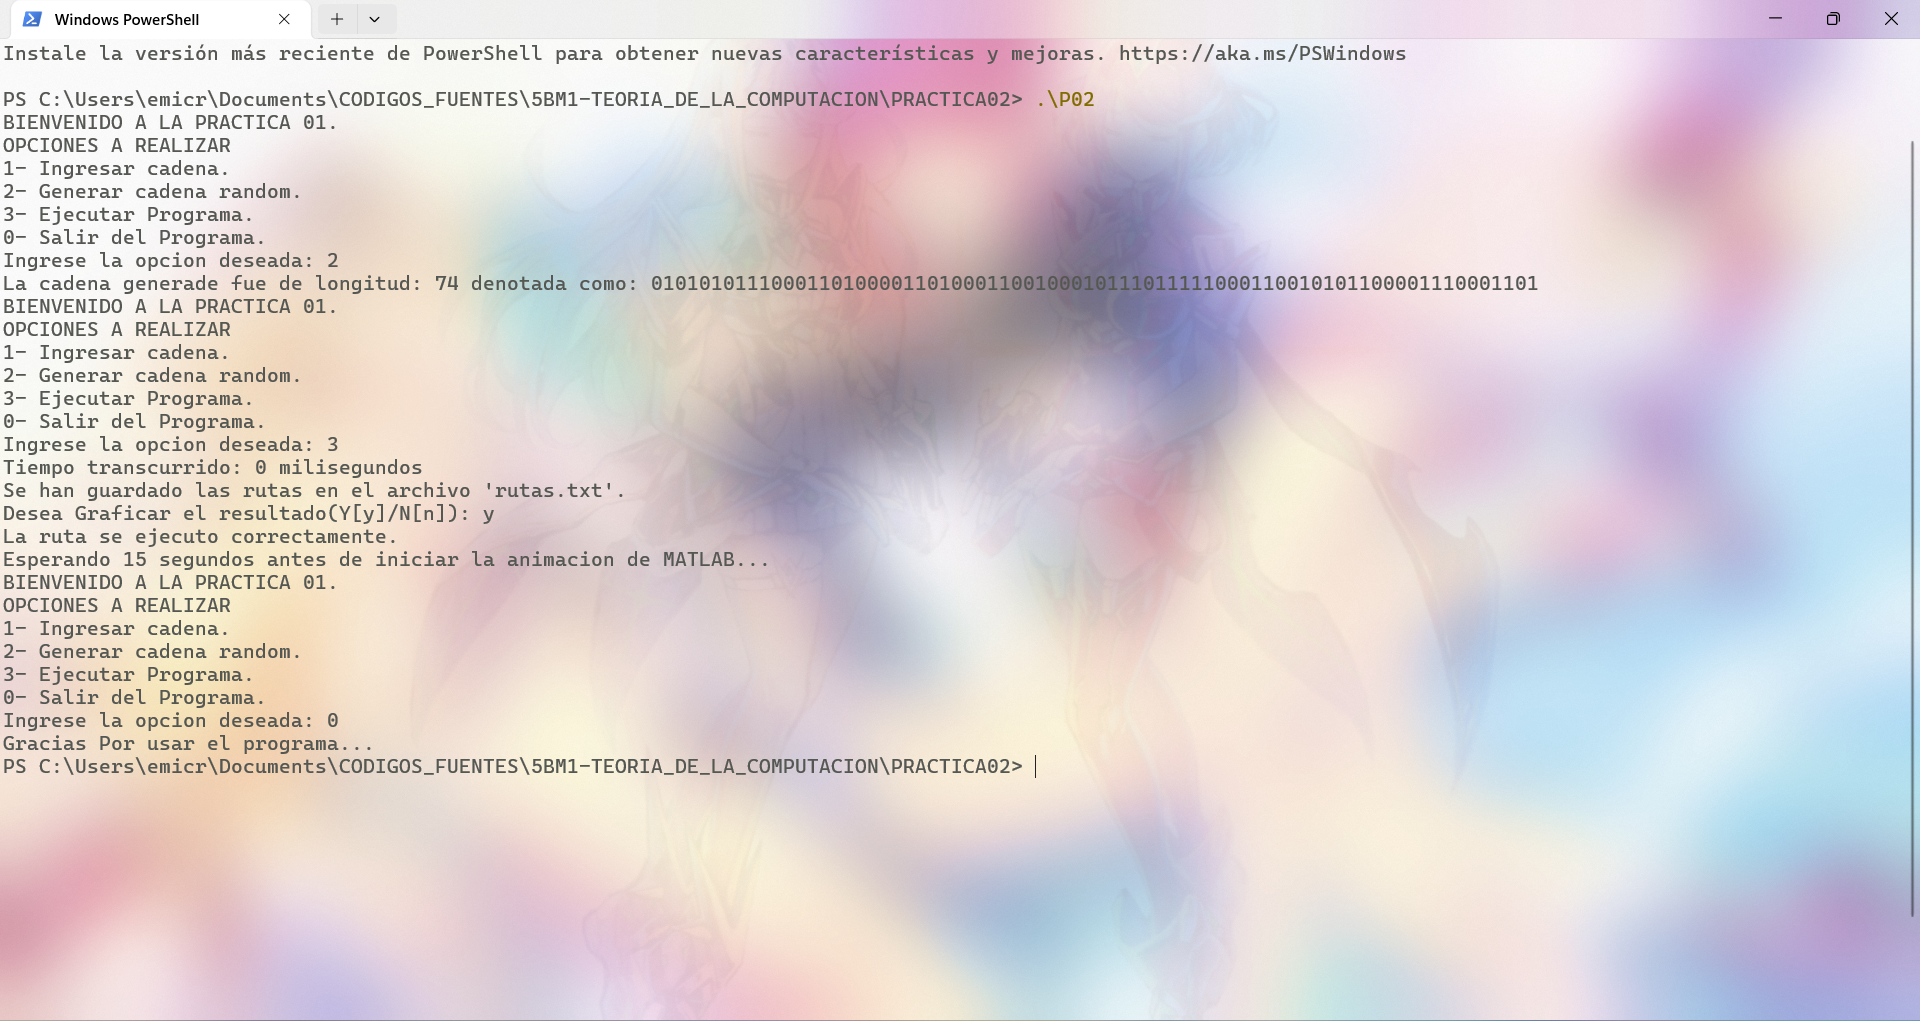
\includegraphics[width=1\linewidth]{Terminal.png}
    \caption{Ejecucion de la Practica 01 en terminal.}\label{Terminal}
\end{figure}

\begin{figure}[H]
    \centering
    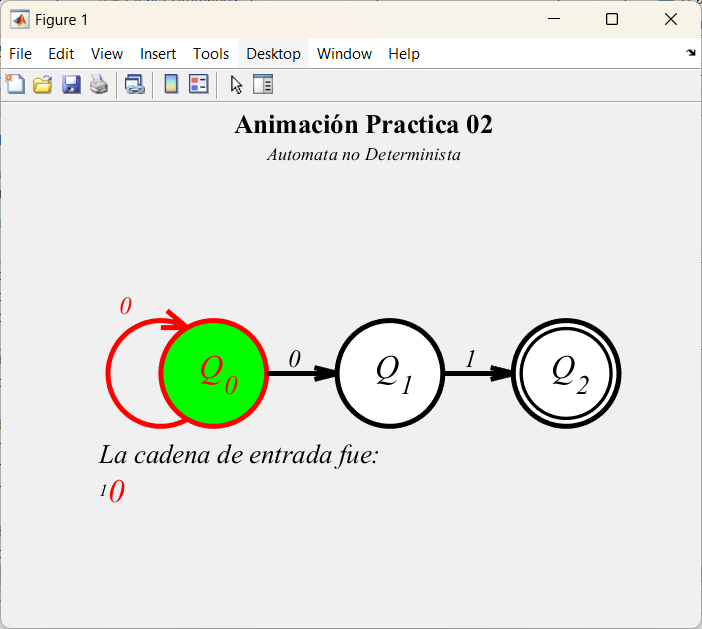
\includegraphics[width=0.7\linewidth]{AutomataQ0.png}
    \caption{Grafico resultante con potencia = 28}\label{AutomataQ0}
\end{figure}

\begin{figure}[H]
    \centering
    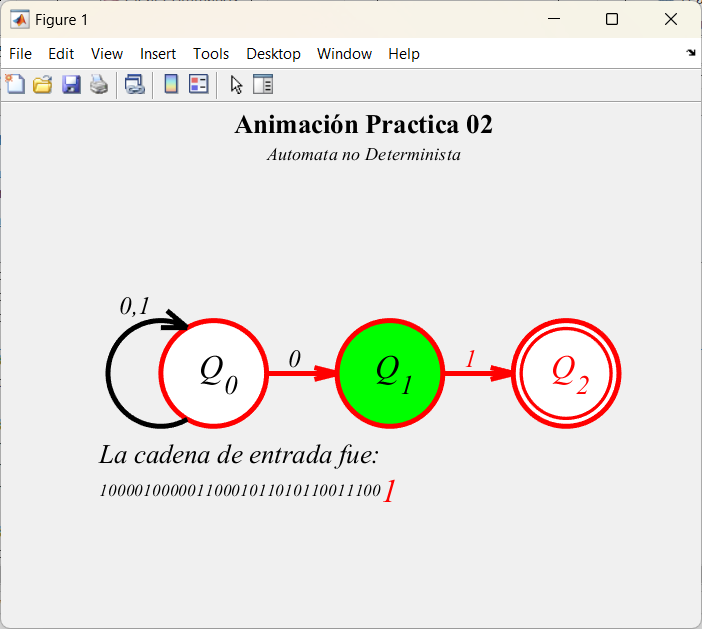
\includegraphics[width=0.7\linewidth]{AutomataQ1.png}
    \caption{Grafico resultante con potencia = 28}\label{AutomataQ1}
\end{figure}

\begin{figure}[H]
    \centering
    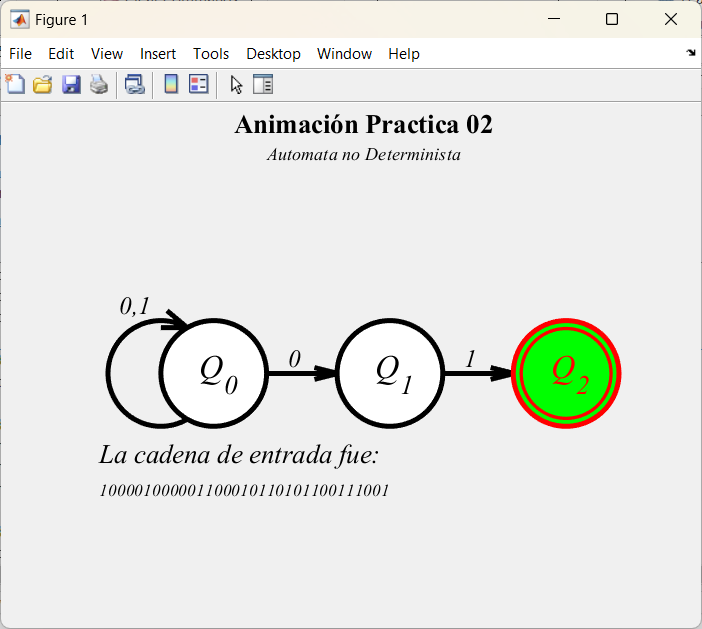
\includegraphics[width=0.7\linewidth]{AutomataQ2.png}
    \caption{Grafico resultante con potencia = 28}\label{AutomataQ2}
\end{figure}

Este es el resultado en el \textit{rutas.txt} con una longitud de setenta y dos:
\begin{lstlisting}[language={},basicstyle=\ttfamily\footnotesize, breaklines=true]
Se encontraron las siguientes rutas para la cadea:
<<01010101110001101000011010001100100010111011111000110010101100001110001101>>:
Ruta: Q0 -> Q0 -> Q0 -> Q0 -> Q0 -> Q0 -> Q0 -> Q0 -> Q0 -> Q0 -> Q0 -> Q0 -> Q0 ->
Q0 -> Q0 -> Q0 -> Q0 -> Q0 -> Q0 -> Q0 -> Q0 -> Q0 -> Q0 -> Q0 -> Q0 -> Q0 -> Q0 ->
Q0 -> Q0 -> Q0 -> Q0 -> Q0 -> Q0 -> Q0 -> Q0 -> Q0 -> Q0 -> Q0 -> Q0 -> Q0 -> Q0 ->
Q0 -> Q0 -> Q0 -> Q0 -> Q0 -> Q0 -> Q0 -> Q0 -> Q0 -> Q0 -> Q0 -> Q0 -> Q0 -> Q0 ->
Q0 -> Q0 -> Q0 -> Q0 -> Q0 -> Q0 -> Q0 -> Q0 -> Q0 -> Q0 -> Q0 -> Q0 -> Q0 -> Q0 ->
Q0 -> Q0 -> Q0 -> Q0 -> Q1 -> Q2

\end{lstlisting}


\section{Conclusiones}
Al completar esta práctica, no solo adquirí conocimientos técnicos en la implementación de algoritmos y la visualización de datos, sino
que experimenté un viaje integral que fusionó la teoría y la práctica en el vasto mundo de la informática. A lo largo de este proceso,
profundicé en los fundamentos de la teoría de autómatas, aplicando conceptos abstractos en la generación de potencias de un alfabeto
utilizando C++. Este ejercicio me permitió no solo entender los principios teóricos detrás de la generación de potencias, sino también
apreciar la importancia de la implementación práctica para comprender plenamente su alcance y aplicación en el mundo real.

Además, al explorar la visualización de datos en MATLAB, descubrí cómo transformar números y conceptos abstractos en imágenes claras y
significativas. La representación gráfica de los datos generados me proporcionó una nueva perspectiva sobre el comportamiento de los
sistemas computacionales, permitiéndome identificar patrones, tendencias y anomalías que de otro modo podrían haber pasado desapercibidos.
Esta experiencia me capacitó para comunicar de manera efectiva los resultados de mis análisis y tomar decisiones informadas basadas en
la evidencia visual.

Más allá de las habilidades técnicas adquiridas, esta práctica me proporcionó una comprensión más profunda de los conceptos
fundamentales que subyacen en el corazón de la computación. Desarrollé una apreciación más amplia de la importancia de la teoría de
autómatas en la construcción y el análisis de sistemas computacionales, así como una comprensión más aguda de cómo la visualización de
datos puede amplificar nuestra capacidad para comprender y tomar decisiones en entornos complejos.

Como conclusion final, puedo decir, esta práctica me equipó con las habilidades y el conocimiento necesarios para abordar desafíos más
complejos en mi viaje en el mundo de la informática y la ciencia de datos. Al integrar teoría y práctica en un viaje de descubrimiento
computacional, avancé hacia un mayor dominio de los principios fundamentales y las herramientas necesarias para enfrentar los desafíos
del futuro con confianza y perspicacia.

\bibliographystyle{ieeetr}
\newpage
\bibliography{referencias}

\end{document}